\section{Proposed questions}

\section*{Part A: Clustering}

\subsection{Question 1}
\textbf{Do clustering-guided summarization alters the behavior and efficacy of the IR system?}

To answer this question we ran the \textbf{clustering based} algorithm using
the same set of documents used in the \textit{first part of the project}. The
result shows a pretty big difference between the two approaches.

% do a minipage fo r2 figurs
\begin{figure}[H]
  \centering
  \begin{minipage}{.5\textwidth}
    \centering
    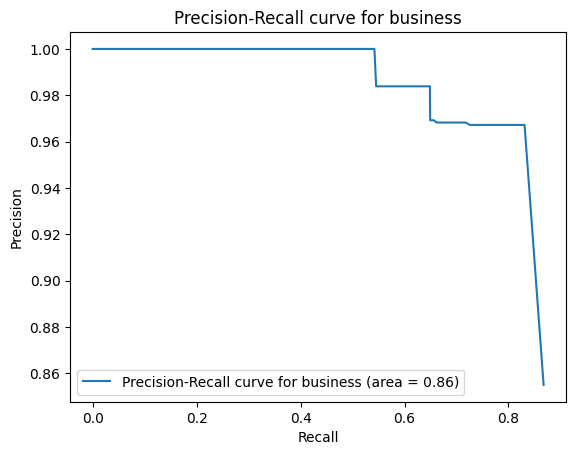
\includegraphics[width=1\linewidth]{images/pr_question_1_part1.png}
    \captionof{figure}{First Part Approach}
    \label{fig:firstpart}
  \end{minipage}%
  \begin{minipage}{.5\textwidth}
    \centering
    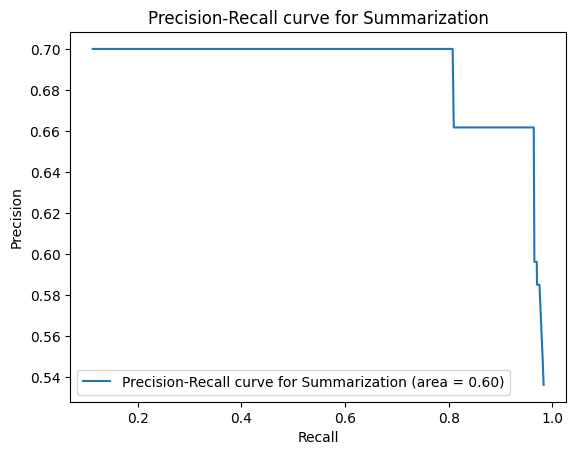
\includegraphics[width=1\linewidth]{images/pr_question_1.png}
    \captionof{figure}{Clustered Approach}
    \label{fig:clustered}
  \end{minipage}
\end{figure}

This result doesn't guarantee that the \textbf{clustering based} approach is
worse than the approach using TFIDF and BM25, because this is based on our
personal implementation of the algorithm. However, it is clear that the
clustering approach is not as effective as the first approach in this case. A
possible way to improve the algorithm could be to consider other sentences
choices rather than focusing on the distance from the centroid of each cluster.

\subsection{Question 2}
\textbf{How sentence representations, clustering choices, and rank criteria impact summarization?}

We benchmarked the performance of the clustering algorithm using a set of
metrics:
\begin{table}[H]
  \centering
  \begin{tabular}{|c|c|c|}
    \hline
    \textbf{Max Clusters} & \textbf{Number of Sentences} & \textbf{Our Metrics} \\
    \hline
    2                     & 3                            &                      \\
    3                     & 5                            &                      \\
    4                     & 7                            & cosine               \\
    6                     & 9                            & euclidean            \\
    8                     & 11                           &                      \\
    10                    & 13                           &                      \\
    \hline
  \end{tabular}
\end{table}

We didn't include any \textbf{different representations} because we only used
the \textbf{TFIDF} representation. The result are indicating a very low
performance of the algorithm using a specific set of metrics.

\begin{table}[H]
  \centering
  \caption{Results of the clustering algorithm using different metrics}
  \label{tab:my-table}
  \begin{adjustbox}{margin={-1cm 0cm 0cm 0cm}}
    \begin{tabular}{|c|c|c|c|c|c|c|c|}
      \hline
      \textbf{\#cluters} & \textbf{\#sentences} & \textbf{metric} & \textbf{avg\_prec} & \textbf{avg\_rec} & \textbf{f1} & \textbf{m\_a\_p} \\ \hline
      2                  & 3                    & cosine          & 0.453504           & 0.449012          & 0.451247    & 0.646069         \\ \hline
      2                  & 3                    & euclidean       & 0.453504           & 0.449012          & 0.451247    & 0.646069         \\ \hline
      2                  & 5                    & cosine          & 0.457060           & 0.633170          & 0.530891    & 0.561392         \\ \hline
      2                  & 5                    & euclidean       & 0.457060           & 0.633170          & 0.530891    & 0.561392         \\ \hline
      2                  & 7                    & cosine          & 0.469898           & 0.768889          & 0.583312    & 0.492352         \\ \hline
      ...                & ...                  & ...             & ...                & ...               & ...         & ...              \\ \hline
      10                 & 9                    & euclidean       & 0.484872           & 0.934921          & 0.638568    & 0.418472         \\ \hline
      10                 & 11                   & cosine          & 0.486431           & 0.941682
                         & 0.641495             & 0.344811                                                                                  \\ \hline
      10                 & 11                   & euclidean       & 0.486431           & 0.941682          & 0.641495    & 0.344811         \\ \hline
      10                 & 13                   & cosine          & 0.486635           & 0.943571          & 0.642110    & 0.336604         \\ \hline
      10                 & 13                   & euclidean       & 0.486635           & 0.943571          & 0.642110    & 0.336604         \\ \hline
    \end{tabular}
  \end{adjustbox}
\end{table}

More insight on this can be found in the \textit{notebook} file.

\subsection{Question 3}
\textbf{ Are anchor sentences (capturing multiple topics) included? And less relevant outlier sen- tences excluded? Justify}

Since our algorithm is based on the \textbf{distance from the centroid} of each
cluster to select the sentences, we are not able to handle the \textbf{anchor
  sentences} and the \textbf{outlier sentences}. We are not able to give a clear
answer to this question, but a possible way to handle this could be to consider
the \textbf{distance from the centroid} and the \textbf{distance from the other
  sentences} inside other clusters. Sentences that are \textbf{more far} from the
centroid of the cluster could be very \textbf{relevant} and could be considered
as \textbf{anchor sentences}, since that sentence could be holding information
between more topics.

\subsection{Question 4}
\textbf{Given a set of documents, plot the distribution of the number of keywords per document. Are keywords generally dissimilar? If not, how would you tackle this challenge?}
For this question we decided to use documents from \textbf{500} to \textbf{700} as range.
The result shows that the distribution of the number of keywords per
document is not uniform.

\begin{figure}[H]
  \begin{minipage}{.5\textwidth}
    \centering
    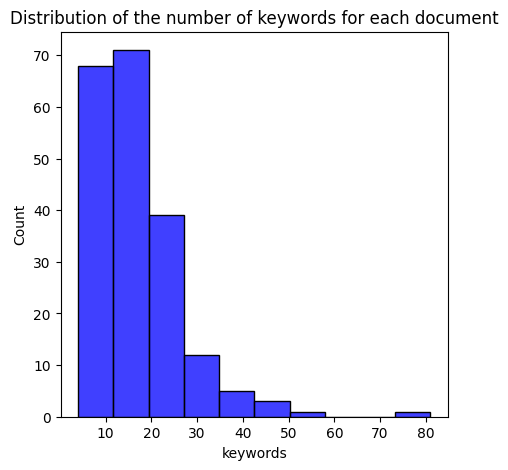
\includegraphics[width=1\linewidth]{images/keyword_distribution.png}
    \captionof{figure}{Distribution of the number of keywords per document}
    \label{fig:question4_1}
  \end{minipage}
  \begin{minipage}{.5\textwidth}
    \centering
    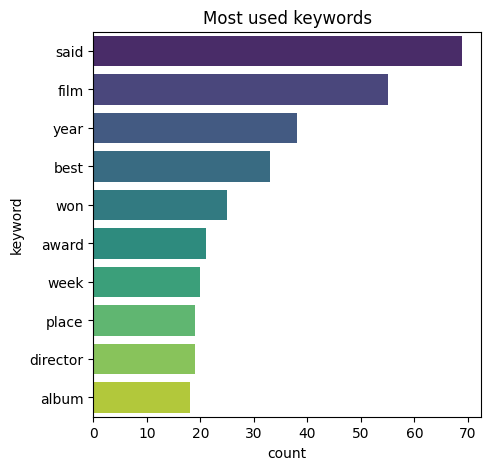
\includegraphics[width=1\linewidth]{images/keyword_distribution_ranks.png}
    \captionof{figure}{Distribution of the number of keywords per document}
    \label{fig:question4_2}
  \end{minipage}
\end{figure}

The main problem is that the \textbf{keywords} are not \textbf{dissimilar} and
this could be a problem for the \textbf{clustering algorithm}. In fact, we can
see that a lot of keywords are repeated in the documents. A possible way to
tackle this challenge could be to use a \textbf{different representation} of
the sentences in the space. Moreover, using multiple documents of the same
category could help to improve the performance of the algorithm since the
keywords are more likely to be repeated in the same category.

\section*{Part B: Supervised IR}
\subsection{Question 1}
\textbf{ Does the incorporation of relevance feedback from ideal extracts significantly impact the performance of the IR system? Hypothesize why is that so.}

We can say that a \textbf{model} that is trained using the \textbf{relevance
  feedback} from the \textbf{ideal extracts} could be a nice approach \textbf{only if} the relevance feedback is \textbf{correct}. This is 
  because the model task is to follow the indications given by the guidance, so if the guidance is wrong, the model will be wrong too. That's 
  not a rule for this project, but it's a general rule for machine learning models.

\subsection{Question 2}
\textbf{ Are the learned models able to generalize from one category to another? Justify.}

To answer this question, we treid to train the model using the \textbf{tech category} as a training set, and 
all the other categories as a test set. We used \textit{Random Forest} as a model, since it was the best between the others.
The results show that the model achieved $\approx 0.69$ as it's best performance and $\approx 0.65$ as it's worst performance. 
This result is not bad, but it's not good either. This happens because each category is different from another, and the set of features 
that we are using may not be the best. However, to \textit{effectively test the model}, what we could do is to train another model 
using a training set of the same size as the \textit{tech category training set}, but using a mixture between all the categories.
In this way we could have a better vision of the model's performance in the generalization task. 


\subsection{Question 3}
\textbf{Which features appear to be more relevant to the target summarization task? Do sentence- location features aid summarization?}

The most important feature that we found is the score given by the \textit{similarity} between the sentence and the document. To get this 
insight, we used a library called \textit{SHAP} that helps us to understand the importance of each feature in the model. It uses the concept of 
\textit{Shapley Values}, a concept from game theory that given a model and a set of features, it assigns to each feature a value that represents
how much the feature contributes to the model's prediction. 

To answer the second part of the question, we can say that the \textit{sentence-location} feature is a good one, because it the 4th most important.

\begin{figure}[H]
  \centering
  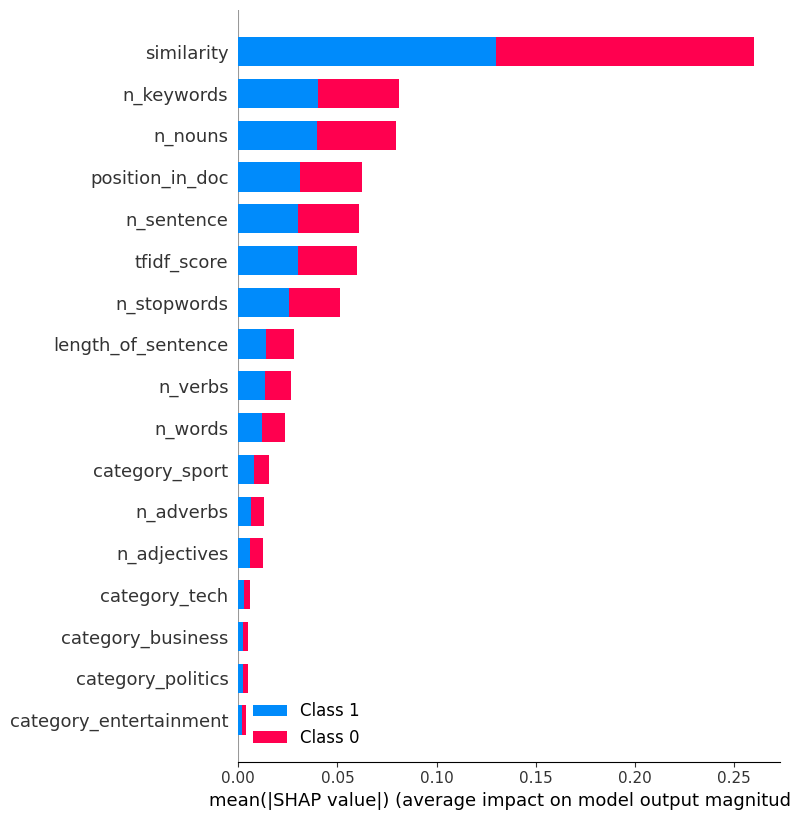
\includegraphics[width=0.5\textwidth]{images/shap.png}
  \caption{SHAP values for the Random Forest model}
  \label{fig:shap_values}
\end{figure}

\subsection{Question 4}
\textbf{In alternative to the given reference extracts, consider the presence of manual abstractive summaries, can supervised IR be used to explore such feedback? Justify}

This question requires a detailed explanation.